\chapter{Software Development Stream Analysis (SDSA)}
\label{ch:Framework}

SDSA is a Hackystat extension that provides a generic framework for 
organizing various kinds of software metrics received by Hackystat 
into a form appropriate as input to a rule-based, time-series analysis 
(Figure \ref{fig:ZorroInfrastructure}). SDSA supports (1) construction 
of software development streams, (2) partition of software development 
streams, and (3) inference of development behaviors. 

The SDSA framework supports completely automated analysis, once configured.
First, the data collection is automated because SDSA uses software process 
metrics collected by Hackystat sensors. The sensors collect in-process software 
metrics automatically and unobtrusively. Second, the construction and 
partitioning of the software development stream is automated. SDSA reduces 
software process metrics into development activities for construction of a 
software development stream, which is then partitioned into episodes. Once 
a development stream has been partitioned into a sequence of episodes, 
SDSA can analyze the development behaviors in these episodes and classify 
them according to whatever process is under analysis. Finally, the inference 
process is also automated because SDSA uses JESS\cite{Friedman-Hill:03}, 
a rule-based system in Java. Developers can specify part or all of the 
studied process as a set of rules. 

The SDSA framework is designed to be customized for a specific software 
process of interest. Developers can selectively choose the event streams
to merge in the software development stream construction phase (see Section
\ref{sec:SDSA-Construction}). For a software process, developers can 
use different tokenizers to partition the development streams (see Section 
\ref{sec:SDSA-Partition}). Also, different rules can be supplied for 
development behaviors inference (see Section \ref{sec:SDSA-Inference}). 

This chapter begins with an introduction to the Hackystat framework
on which the SDSA framework is built, followed by a description
of the SDSA framework itself. 

%The SDSA framework reduces a series of
%software metrics into an event stream, generate software development
%stream by merging event streams 
%%Low-level software processes emphesizes on software developers. They
%%carry out software projects following best practices and guideline 
%%provided by the low-level software processes. 

\section{Hackystat}
Hackystat is an open source framework for automated collection and analysis
of software engineering process and product metrics. Hackystat supports 
unobtrusive data collection via specialized ``sensors'' that are attached 
to development environment tools. These sensors send structured ``sensor 
data type'' instances via SOAP to a web server for analysis via server-side 
Hackystat ``applications''. Over two dozen sensors are currently available, 
including sensors for IDEs (Emacs, Eclipse, Vim, VisualStudio, Idea), 
configuration management (CVS, Subversion), bug tracking (Jira, Bugzilla), 
testing and coverage (JUnit, CppUnit, Emma, JBlanket), 
system builds and packaging (Ant), 
static analysis (Checkstyle, PMD, FindBugs, LOCC, SCLC), and so forth.

Hackystat is tool, environment, and process independent. It does not 
presume a specific operating system platform, a specific integrated 
development environment, or a specific software process. It is designed
to be extensible. It provides not only generic services such as 
software metrics collection, persistence and retrieval, and project 
definition management for conglomerating discrete software metrics 
from both an individual and other project members, but also an 
extension mechanism where new modules (sensors or applications) 
can be added. Applications of the Hackystat framework in addition 
to SDSA include in-process project management \cite{csdl2-04-11}, high 
performance computing \cite{csdl2-04-22}, and software engineering
education \cite{csdl2-03-12}.

\subsection{Software Metrics Collection, Persistence, and Retrieval}
When developers are programming in a development environment tool with
its sensor installed and enabled, the sensor will collect both
the process and product metrics unobtrusively. The sensors then send
them via SOAP to a web server that hosts Hackystat.
The architecture of Hackystat is client-server. The \textit{``clients''} 
can be development environment such as Emacs, Eclipse, 
and Microsoft Visual Studio. The \textit{``server''} is the 
framework itself and its extended applications. On the server-side
Hackystat handles metrics data persistence automatically. It stores 
them in XML formats and implements a self-managed caching mechanism 
to retrieve them when requested by the applications. 

\subsection{Extension Mechanism}
The Hackystat system provides an extension mechanism to support new 
functionalities including sensor data types (metrics), sensors, 
applications, documentation, and so forth. Each functionality needs 
to specify a configuration file in XML saying what it is about and 
what part of Hackystat it will extend. For instance, if you are developing a 
new sensor for the Java development environment tool NetBeans, you 
will specify a sensor definition file such as netbeans.sensor.def.xml. 
It will include the sensor name and
what metrics it collects. The further information on how to implement 
an extended functionality can be found at the Hackystat home 
page:\textit{http://www.hackystat.org}. 

\section{SDSA Framework}
SDSA is an application extending the Hackystat framework. It organizes
various kinds of process metrics data into a time-series software 
development stream and conducts rule-based analyses. SDSA is
data oriented. Figure \ref{fig:SDSA-Workflow} illustrates its data model
and work flow. 
\begin{figure}[htbp]
  \centering
  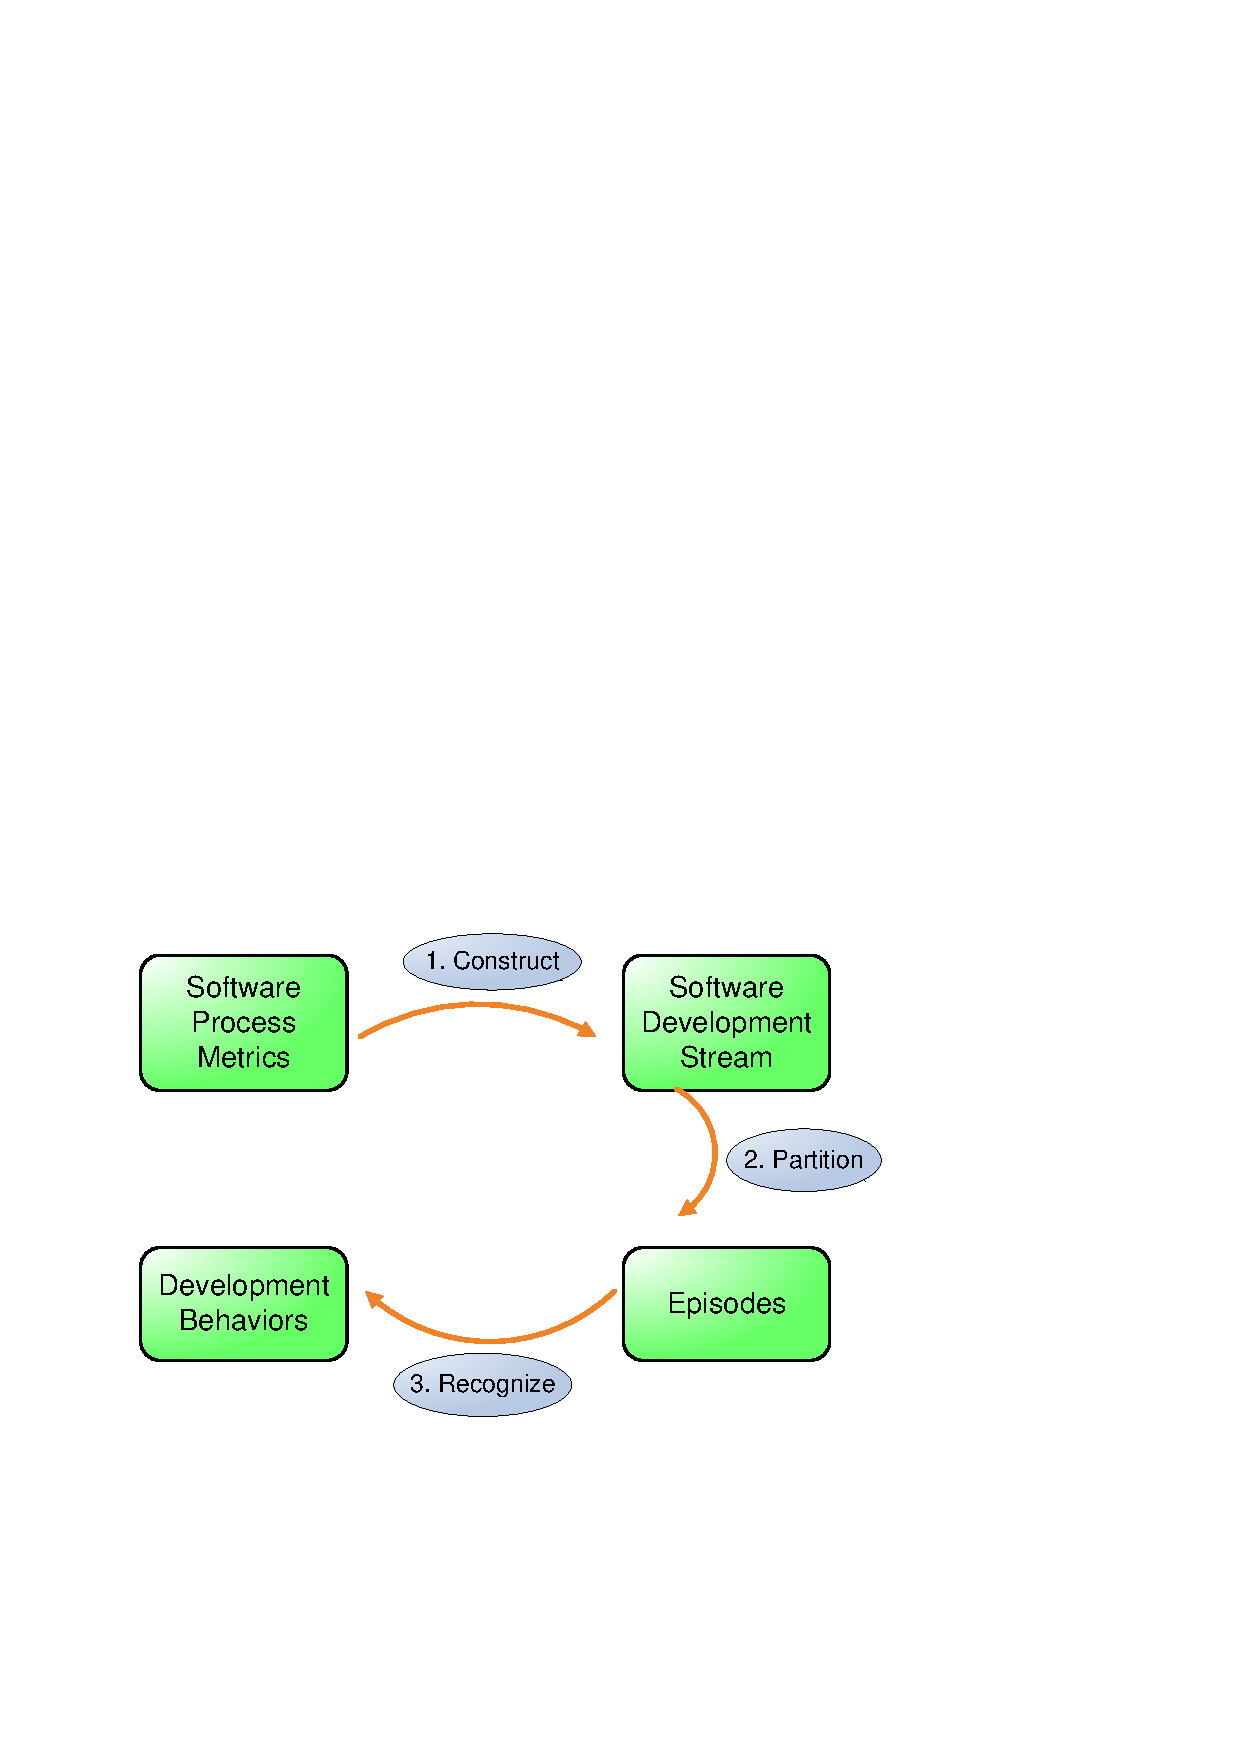
\includegraphics[width=0.5\textwidth]{figs/Visio-SDSA-FlowChart}
  \caption{Data Model and Work Flow of the SDSA Framework}
  \label{fig:SDSA-Workflow}
\end{figure}

SDSA models a software development process as a software development 
stream, which is a time-series data structure consisting of
continuous software development activities collected by Hackystat
sensors. The development stream 
is then partitioned into episodes delimited by boundary conditions. 
Each episode is a data model that represents an atomic components of 
the software process of interest. Eventually, the goal of SDSA is to 
recognize the development behaviors embodied within each episode. 

The data model breaks down the SDSA framework into three 
components(Figure \ref{fig:SDSA-Workflow}): (1) a software 
development stream construction subsystem, (2) a software 
development stream partition subsystem, and (3) a development 
behavior inference subsystem. 

\subsection{Software Development Stream Construction}
\label{sec:SDSA-Construction}
SDSA begins with the development stream construction subsystem 
that translates variety kinds of software process and product 
metrics into a development stream. Figure 
\ref{fig:SDSA-DevelopmentStream} illustrates the process
of software development stream construction. 
\begin{figure}[htbp]
  \centering
  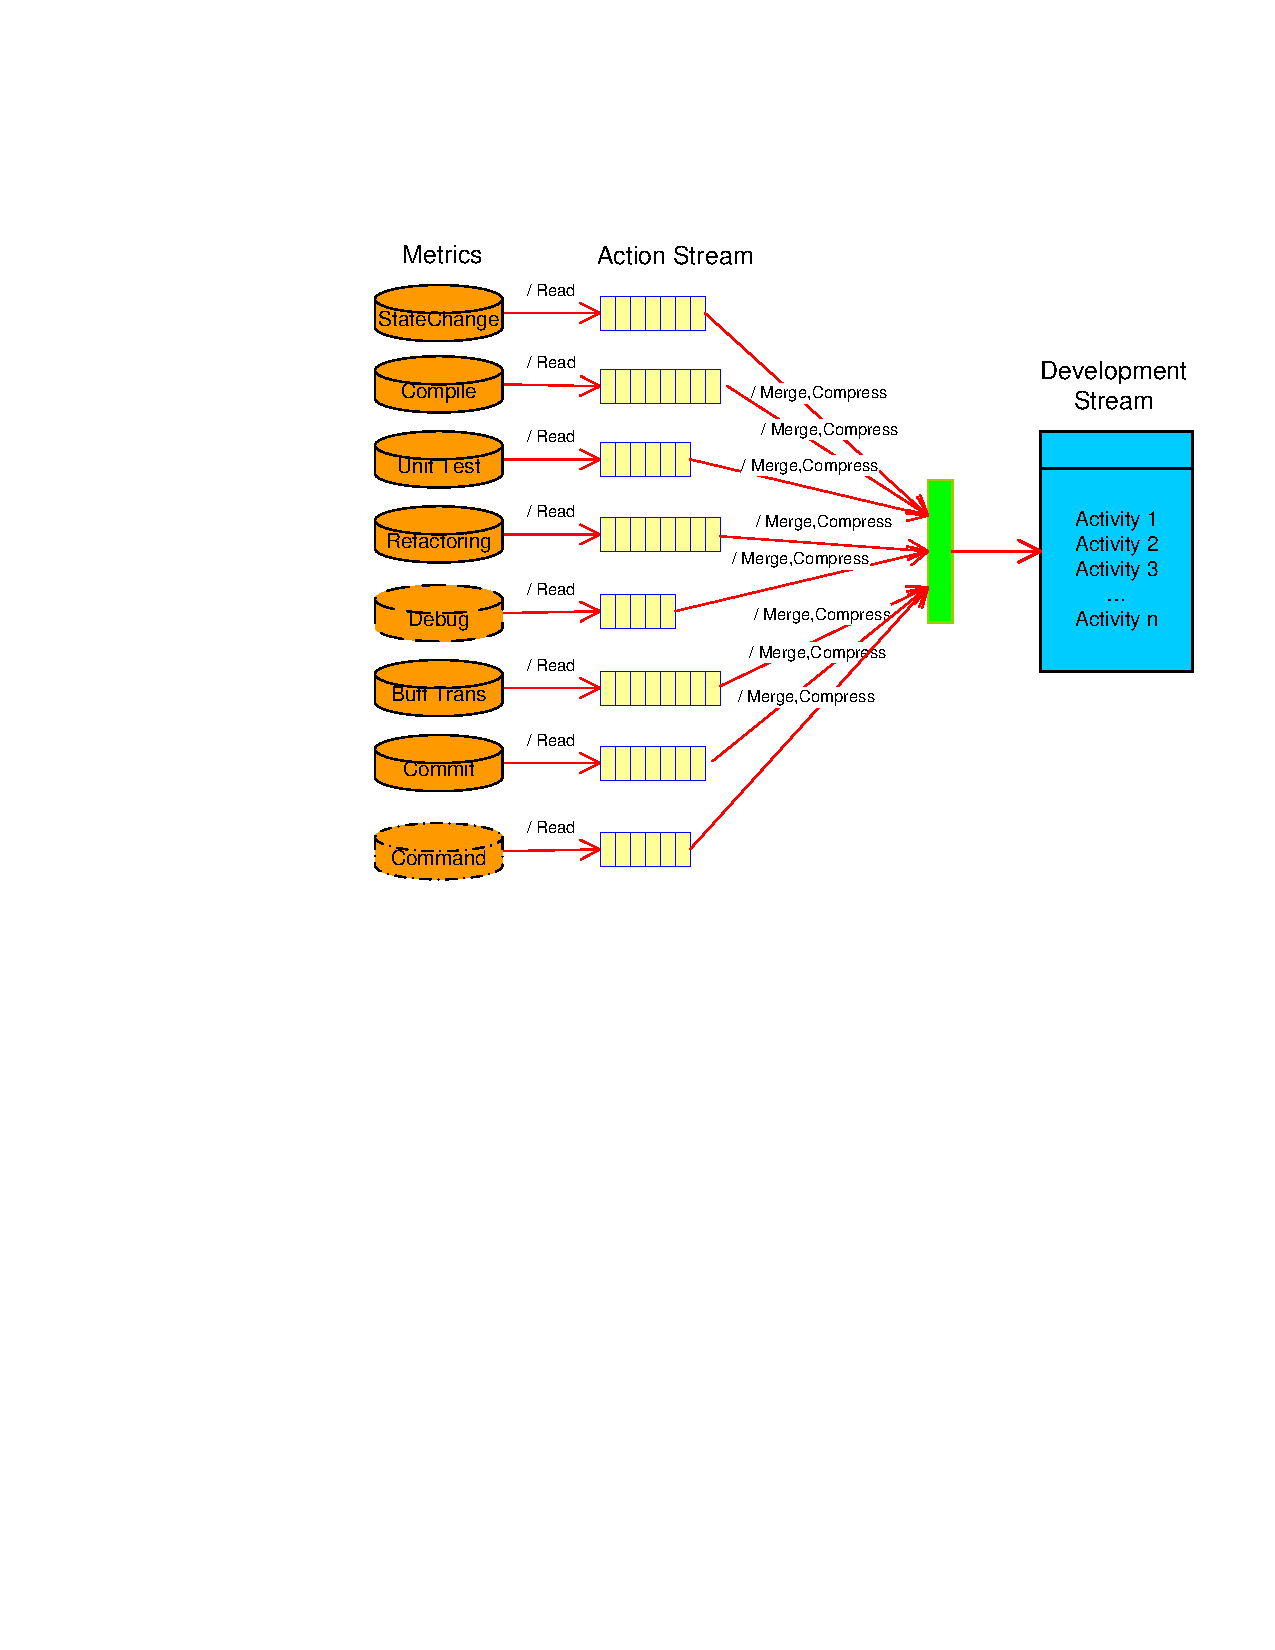
\includegraphics[width=0.8\textwidth]{figs/Visio-SDSA-DevelopmentStream}
  \caption{Software Development Stream Construction}
  \label{fig:SDSA-DevelopmentStream}
\end{figure}

Hackystat sensors collect the software process and product
metrics and abstract them as the structured ``sensor data type''. 
A sensor data entry represents a development activity or an
in-process product metric change that has been caused by a development 
activity. Because sensor data mixes software process and product 
metrics, SDSA must restructure them as development actions in order 
to infer the development behaviors. The development action is 
SDSA's internal representation of the software development 
activities that are collected by Hackystat sensors. 

\subsubsection{Development Action}
Figure \ref{fig:SDSA-Action-UML} is the class diagram of variety of 
development actions SDSA abstracted. All the development actions 
are subtypes of the ``Action'' type. Each action has a clock 
attribute indicating when it occurs and a duration attribute 
indicating how much time it takes. 

\begin{figure}[htbp]
  \centering
  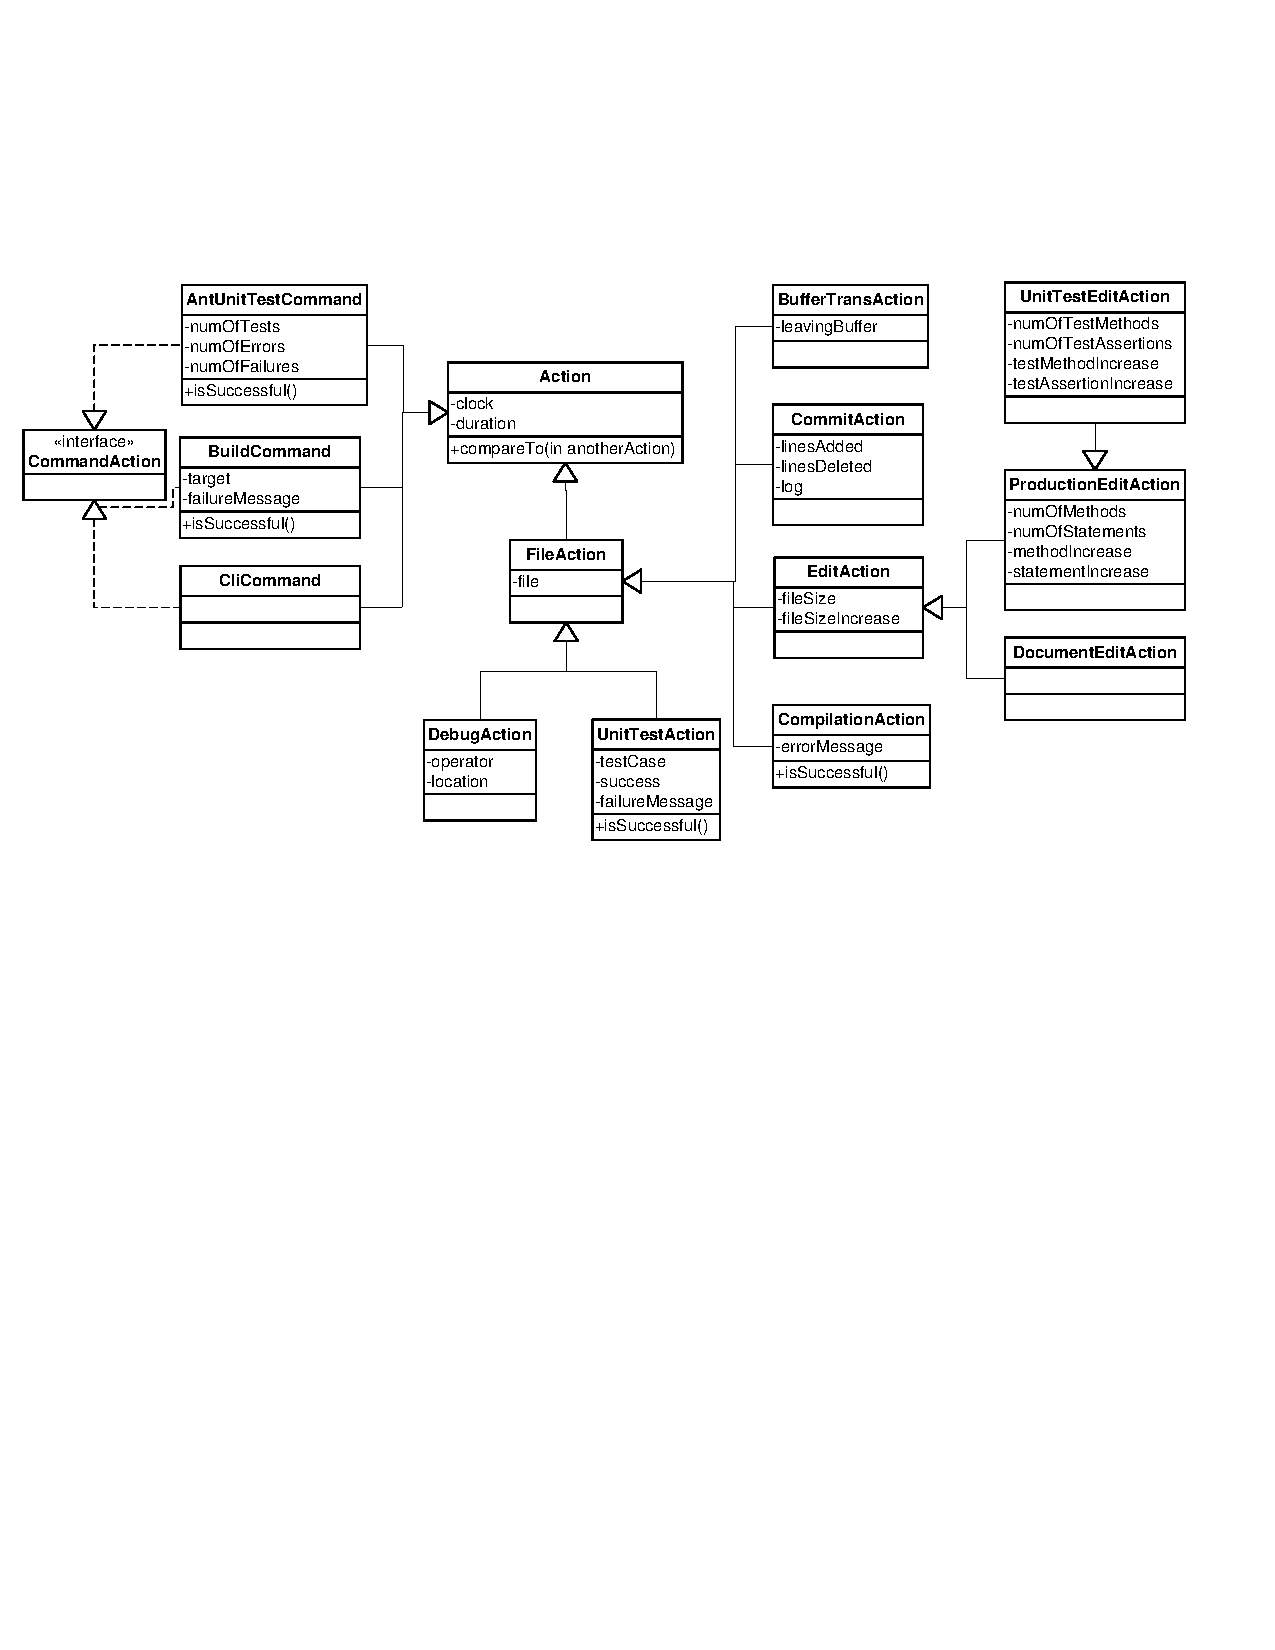
\includegraphics[width=0.9\textwidth]{figs/Visio-Action-UML}
  \caption{Class Diagram of Development Actions}
  \label{fig:SDSA-Action-UML}
\end{figure}

After reading the software metrics of a sensor data type, SDSA 
transforms them into development actions, and then forms 
a time-series action stream.

\subsubsection{Action Stream}
Figure \ref{fig:SDSA-ActionStream-UML} illustrates the class 
diagram of action streams. The ``DataStream'' is the super class 
of all action stream classes. Each action stream has the 
capability of transforming a type of sensor data into a 
time-series action stream. 

\begin{figure}[htbp]
  \centering
  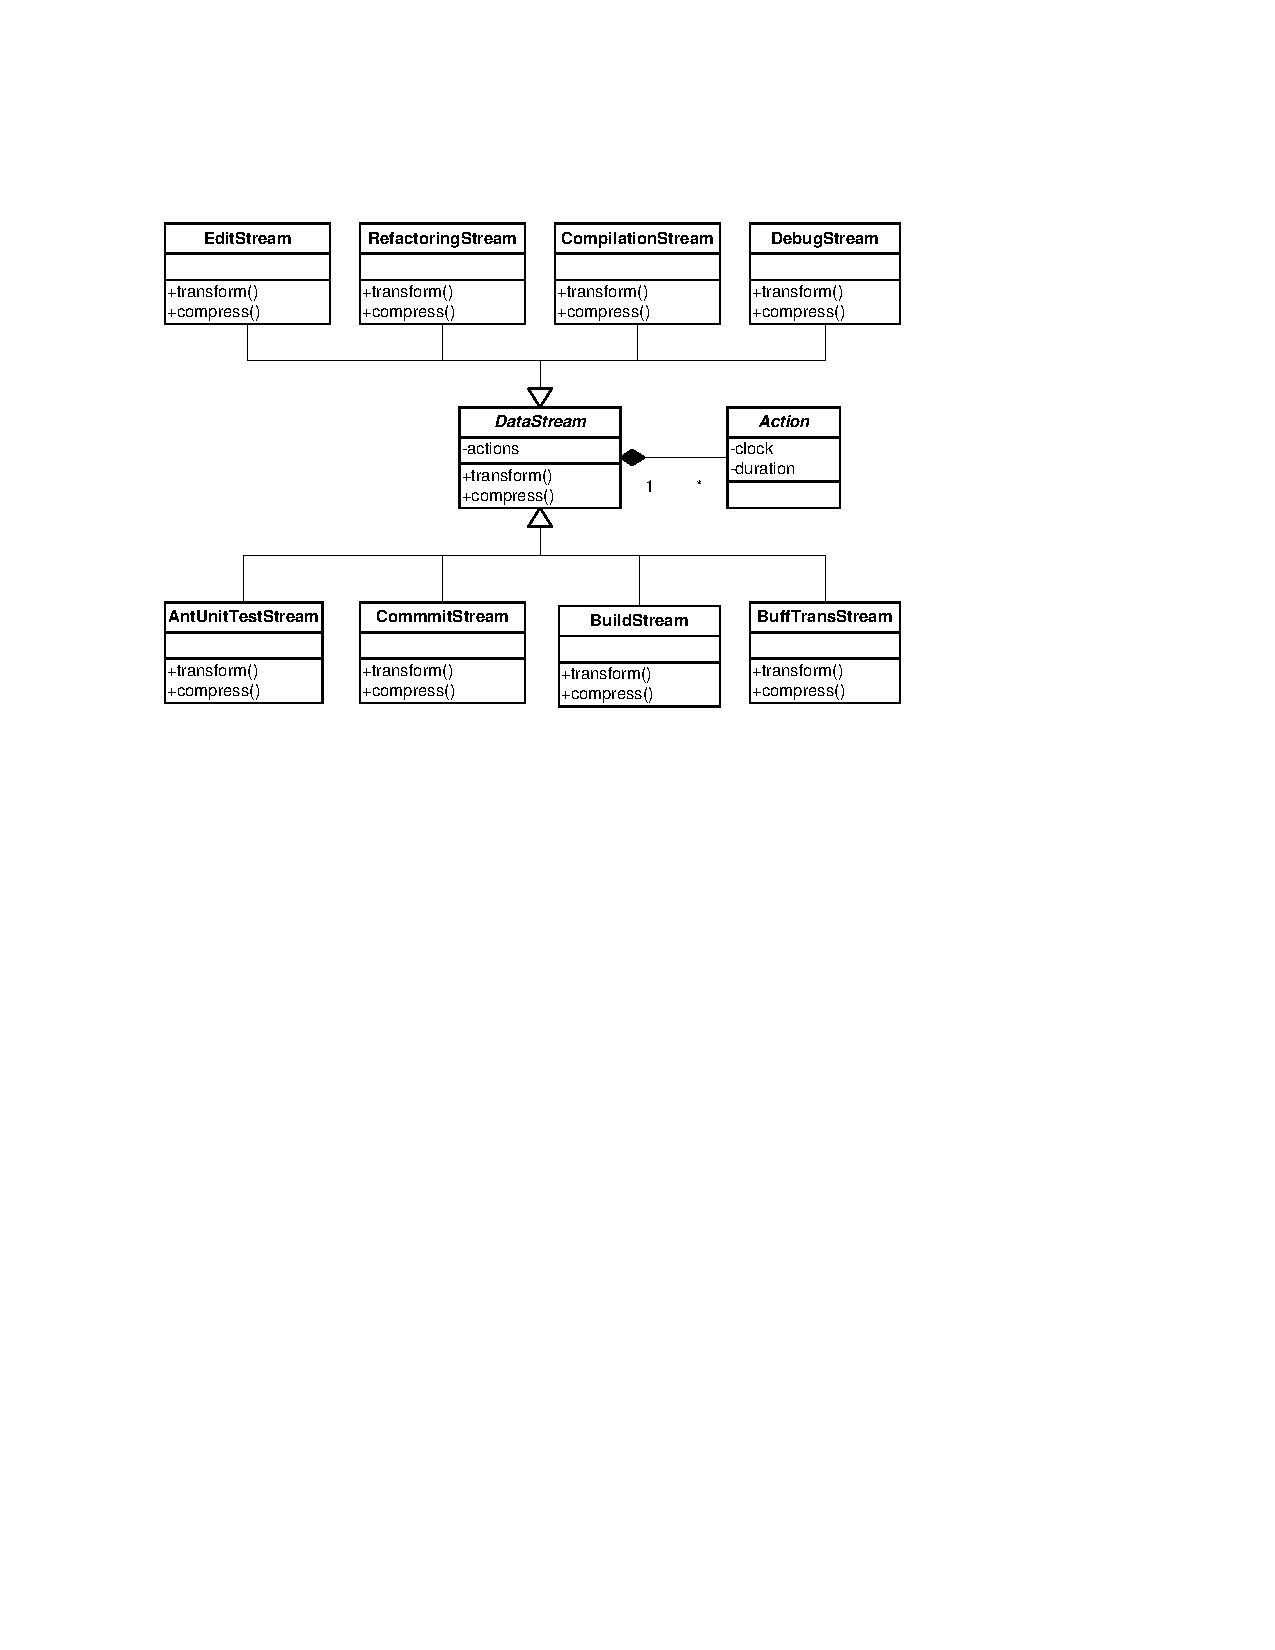
\includegraphics[width=0.8\textwidth]{figs/Visio-ActionStream-UML}
  \caption{Class Diagram of Action Streams}
  \label{fig:SDSA-ActionStream-UML}
\end{figure}

In addition to converting sensor data into development actions, 
an action stream can implement a callback function to compress 
itself. This function can group a set of continuous sensor data 
that represents a single development action. Using unit test 
invocation in the Eclipse IDE as an example, the Eclipse sensor 
collects and sends 3 ``UnitTest'' sensor data entries if the 
invoked unit test has 3 test cases. Because they are the 
consequence of a unit test invocation, the UnitTestStream 
can implement a compress function to group them into a single 
``UnitTest'' development action. 

\subsubsection{Development Stream}
Many kinds of action streams from a developer over a time 
period can merge together to form a software development stream 
as illustrated in Figure \ref{fig:SDSA-DevelopmentStream}. The 
``DevelopmentStream'' is an object representing a software
development stream. It is the container of action streams. The 
following code demonstrates the usage of ``DevelopmentStream''
class. Table \ref{tab:SDSA-StreamExample} is an example that shows
a software development stream's internal representations. 
\begin{verbatim}
   DevelopmentStream stream = 
       new DevelopmentStream(project, user, startDay, endDay);
   stream.addSubstream(new EditStream(user));
   stream.addSubstream(new BuffTransStream(user));
   stream.addSubstream(new RefactoringStream(user));
   stream.addSubstream(new UnitTestStream(user));
   stream.addSubstream(new CompilationStream(user));
   stream.assemble(); 
\end{verbatim}
\begin{table}[htbp]
  \caption{An Excerpt of a Software Development Stream}
  \begin{tabular}{|llll|} \hline
Time & File & Event & Metrics \\ \hline
12:35:29 & TestBowlingGame.java  & ADD METHOD  &	void TestGameCreation() \\ 
12:37:47 & TestBowlingGame.java  & TEST EDIT 	& 120sec MI=+1(3),SI=+1(4),TI=+1(3),AI=0(1) \\ 
12:38:07 & BowlingGame.java &	ADD CLASS &	BowlingGame.java \\ 
12:38:08 & BowlingGame.java &	BUFFTRANS &	FROM TestBowlingGame.java \\ 
12:38:13 & TestBowlingGame.java &	BUFFTRANS &	FROM BowlingGame.java \\ 
12:39:17 & TestBowlingGame.java &	TEST EDIT &	0sec MI=0(3),SI=-1(3),TI=0(3),AI=0(1) \\ 
12:39:17 & TestBowlingGame.java &	COMPILE &	The constructor Frame() is undefined \\
12:39:28 & BowlingGame.java &	ADD METHOD &	BowlingGame(Frame)\\
12:39:30 & BowlingGame.java &	BUFFTRANS &	FROM TestBowlingGame.java\\
12:39:35 & TestBowlingGame.java &	BUFFTRANS &	FROM BowlingGame.java\\
12:39:48 & BowlingGame.java &	PRODUCT EDIT &	0sec MI=+1(1),SI=0(0),FI=+124(124)\\
12:39:50 & BowlingGame.java &	BUFFTRANS &	FROM TestBowlingGame.java\\ \hline
  \end{tabular}
  \label{tab:SDSA-StreamExample}
\end{table}

\begin{comment}
Hackystat sensors can collect many kinds of software process metrics
including editing, compilation, unit testing, refactoring, and 
so forth. SDSA transforms these software metrics into development
events and builds event streams out of them. A development event
in SDSA has basic information such as time stamp, the target file,
duration etc. An event stream collects and sorts the development 
events from a kind in time sequence. Developers can select event
streams to merge for creating the software development stream (SDS). 

For example, the ``State Change'' sensor data type is 
an innovative approach collecting developer' editing activities in a
development environment indirectly. As a result, an editing activity
can be represented by one or several ``State Change'' sensor data
entries. 


The SDS is an abstraction of time-series software development events. 
One purpose of SDSA is to mine the sequential development streams to 
understand executions of low-level software processes. The data-driven 
methods are amenable for analyzing SDS because it has massive 
development events. Machine Learning (ML) \cite{} is a very popular
data-driven method. 

Data-Driven
To understand the software process
behind a software development stream, one can easily think of
machine learning \cite{}. It has already been widely used in 
the pattern recognition and data classification in data mining
and bioinformatic research \cite{}. Some research \cite{} already 
studied how it can be used for understanding time-series data. 
Cook demonstrated in his research that the machine learning 
algorithms can potentially discover and validate software 
processes. Furthermore, the machine learning technique can be 
more effective in understanding data if it is being supervised. 

Goal-Driven

Software process research is typical top-down. The goal-driven
GQM software engineering paradigm. Simulating how a process
model can be adapted in the real situation is a standard 
research method \cite{}. 

Both data-driven and goal-driven research methods have their 
pros and cons. Data-Driven suffer local minimization or 
over fitting problems. Goal-Driven is too ideal to be applied
in the real settings. The process experts have to be hired 
to enforce the process data collection and analysis. In my 
research, I proposed to take a trade-off between the goal-driven
and data-driven research paradigms. As a result of my research, 
I came up with a marriage of software development stream
and episode behavior inference. 
\end{comment}

\subsection{Software Development Stream Partition}
\label{sec:SDSA-Partition}
The second component of SDSA is the software development stream 
partition subsystem. 
The software development stream is a time-series data structure
that may have hundreds to thousands development activities. Though
applying machine learning algorithm is plausible \cite{Cook:95}, 
I proposed a mechanism to partition the development streams into 
episodes using the boundary conditions (Figure \ref{fig:SDSA-Partition}).
\begin{figure}[htbp]
  \centering
  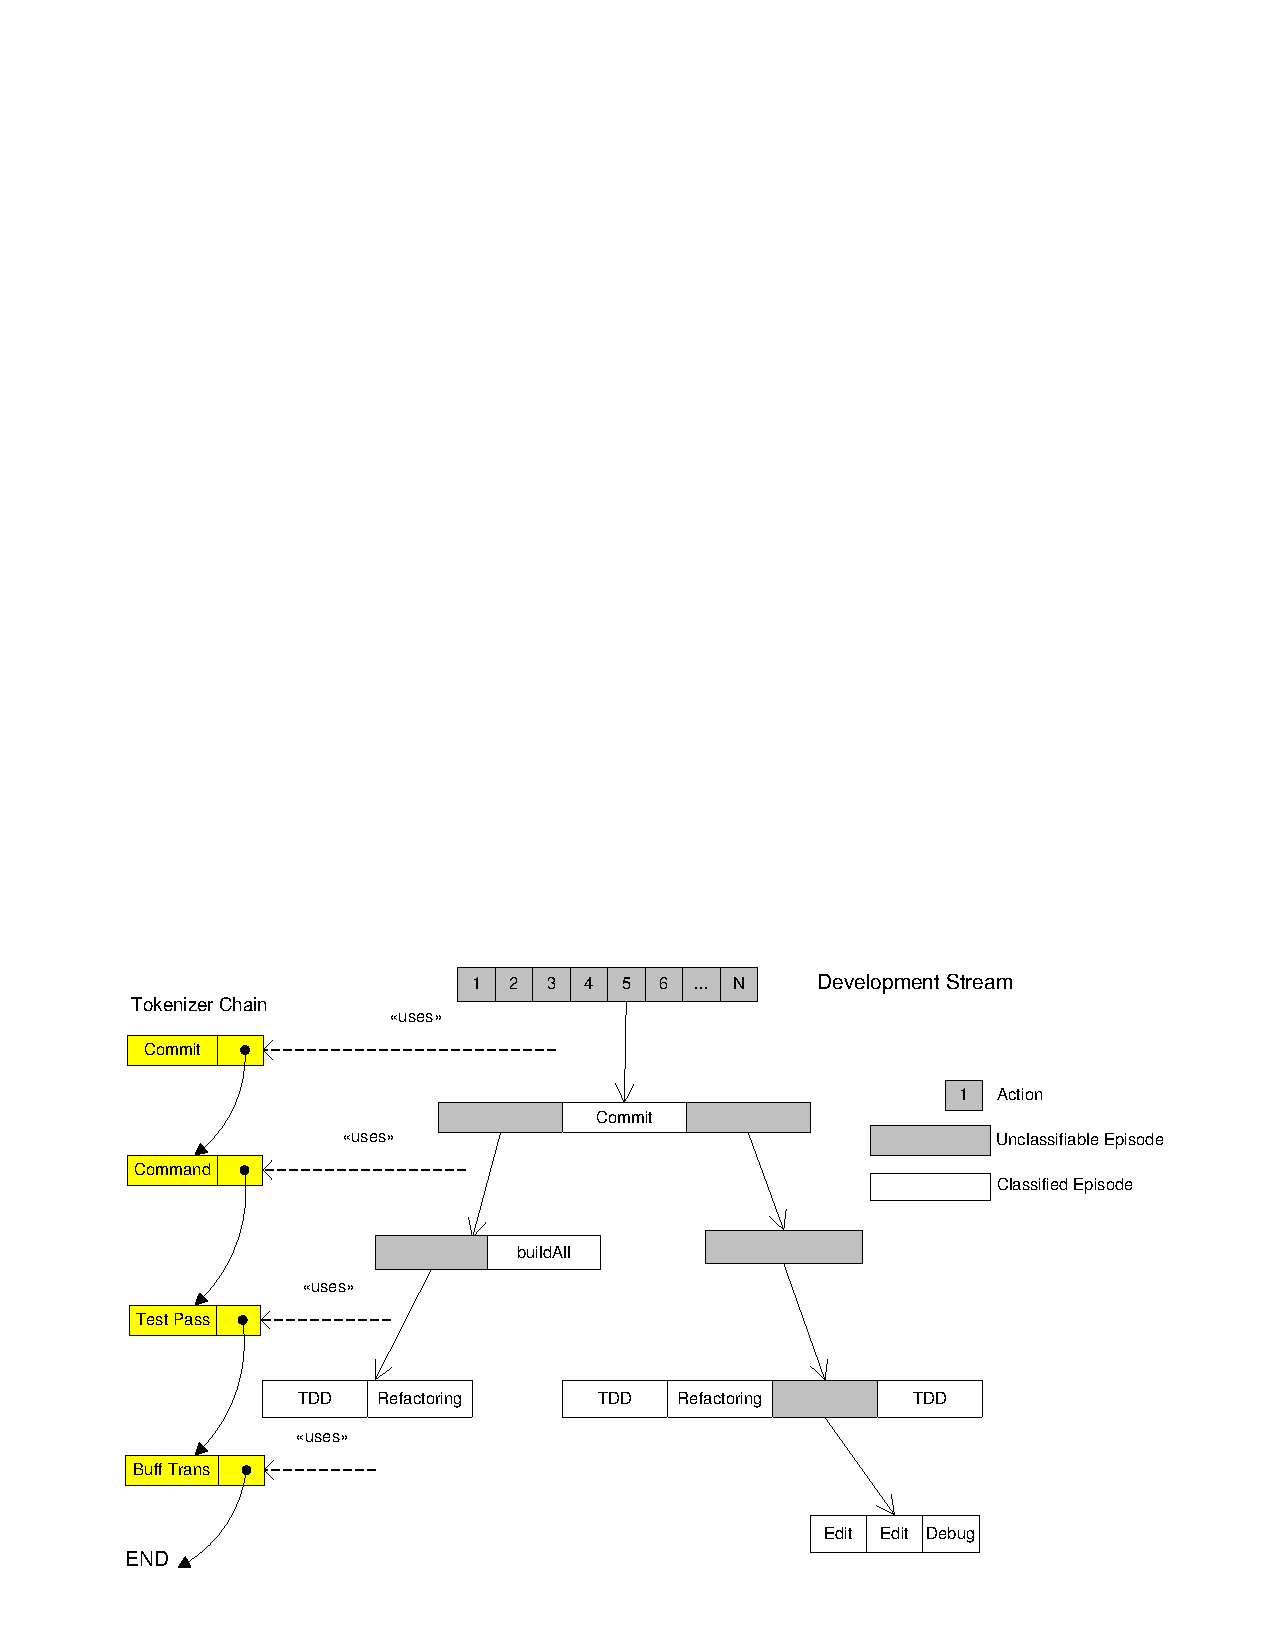
\includegraphics[width=0.8\textwidth]{figs/Visio-SDSA-Partition-UML}
  \caption{Partition of Development Stream}
  \label{fig:SDSA-Partition}
\end{figure}

Larman and Basili\cite{Larman:03} claim that the software development 
is iterative and incremental. Thus, tokenizing development streams not 
only simplifies mining large volumes of data, but also provides an approach 
to comparing actual software development processes to software process 
theories. Figure \ref{fig:SDSA-Partition} illustrates 
the design of the software development stream partition algorithm. 
Tokenizers, which partition software development streams using 
boundary conditions, can be chained together. Currently, four tokenizers 
have been developed in SDSA. Figure \ref{fig:SDSA-Tokenizers} illustrates 
their class diagram. Of course, developers can implement and add 
new tokenizers if necessary. 
\begin{itemize}
\item {\textbf{Commit Tokenizer}} partitions development streams by
source code repository commit actions.  

\item {\textbf{Command Tokenizer}} partitions development streams by
commands invoked in a shell window. 

\item {\textbf{Test Pass Tokenizer}} partitions development streams
by successful unit test invocations. 

\item {\textbf{Buffer Transition Tokenizer}} partitions development
streams by buffer changes in an IDE. 
\end{itemize}
\begin{figure}[htbp]
  \centering
  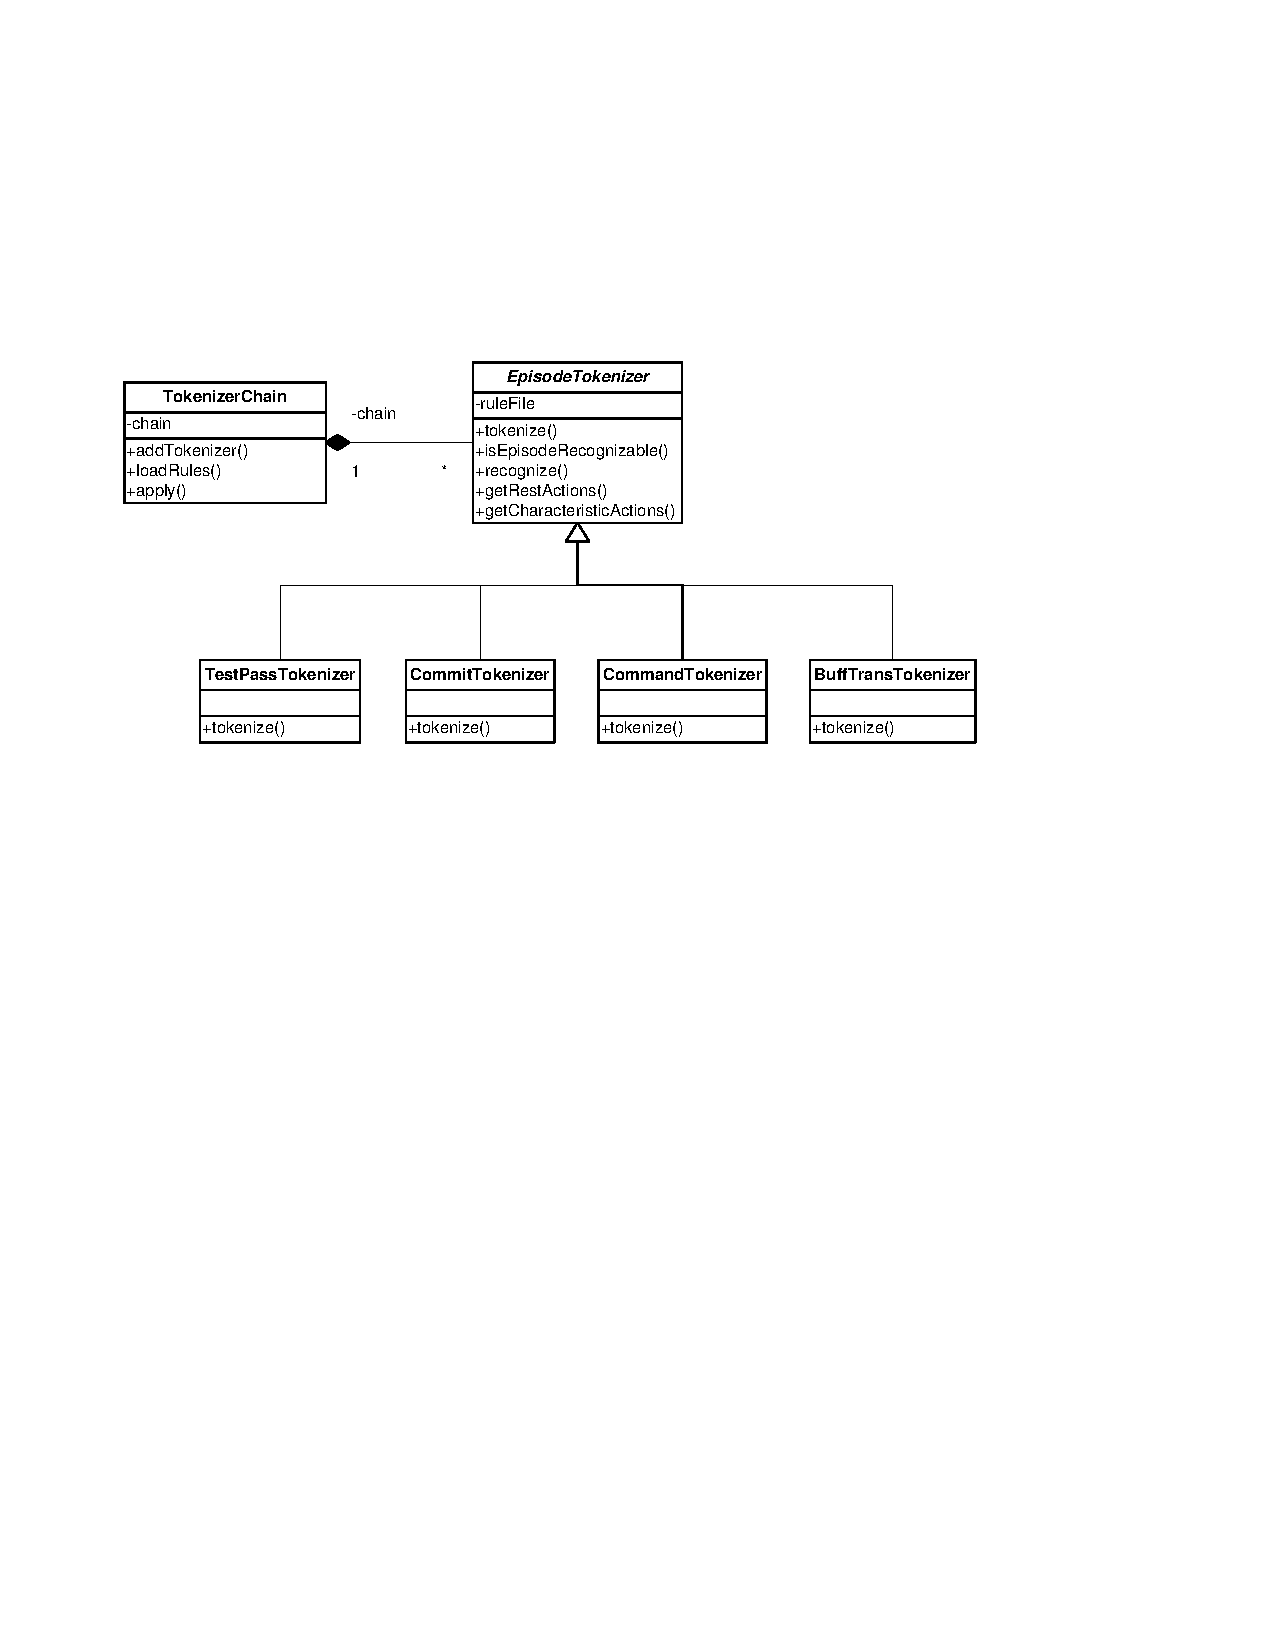
\includegraphics[width=0.8\textwidth]{figs/Visio-SDSA-Tokenizers-UML}
  \caption{Class Structure of SDSA Tokenizers}
  \label{fig:SDSA-Tokenizers}
\end{figure}

Although it is possible, it is not necessary to have multiple
tokenizers in a single run. In my dissertation research, I found that 
the ``test pass'' tokenizer is sufficient for the inference of 
Test-Driven Development behaviors.

% A software development stream could have thousands activities.
% It is hard to and time-consuming to analyeze a development stream
% which may have ton of activities. And, very likely, there is no
% any connection between a activity and another activities that is
% days or months away. So I decided to partition software 
% development streams. By using tokenizer, we may be able to cut
% them into chunks having activities that are clsey tied with
% each other. 
\subsection{Development Behaviors Inference}
\label{sec:SDSA-Inference}
SDSA infers development behaviors using JESS \cite{Friedman-Hill:03}, 
a rule-based system. Figure \ref{fig:SDSA-Inference} illustrates 
how SDSA interacts with JESS to infer development behaviors from
development actions in an episode. 
% regognition of Low-level Software Process Behaviors
% Utilize JESS, a rule-based system to look for and match
% the pattern of software development in episodes. 
\begin{figure}[htbp]
  \centering
  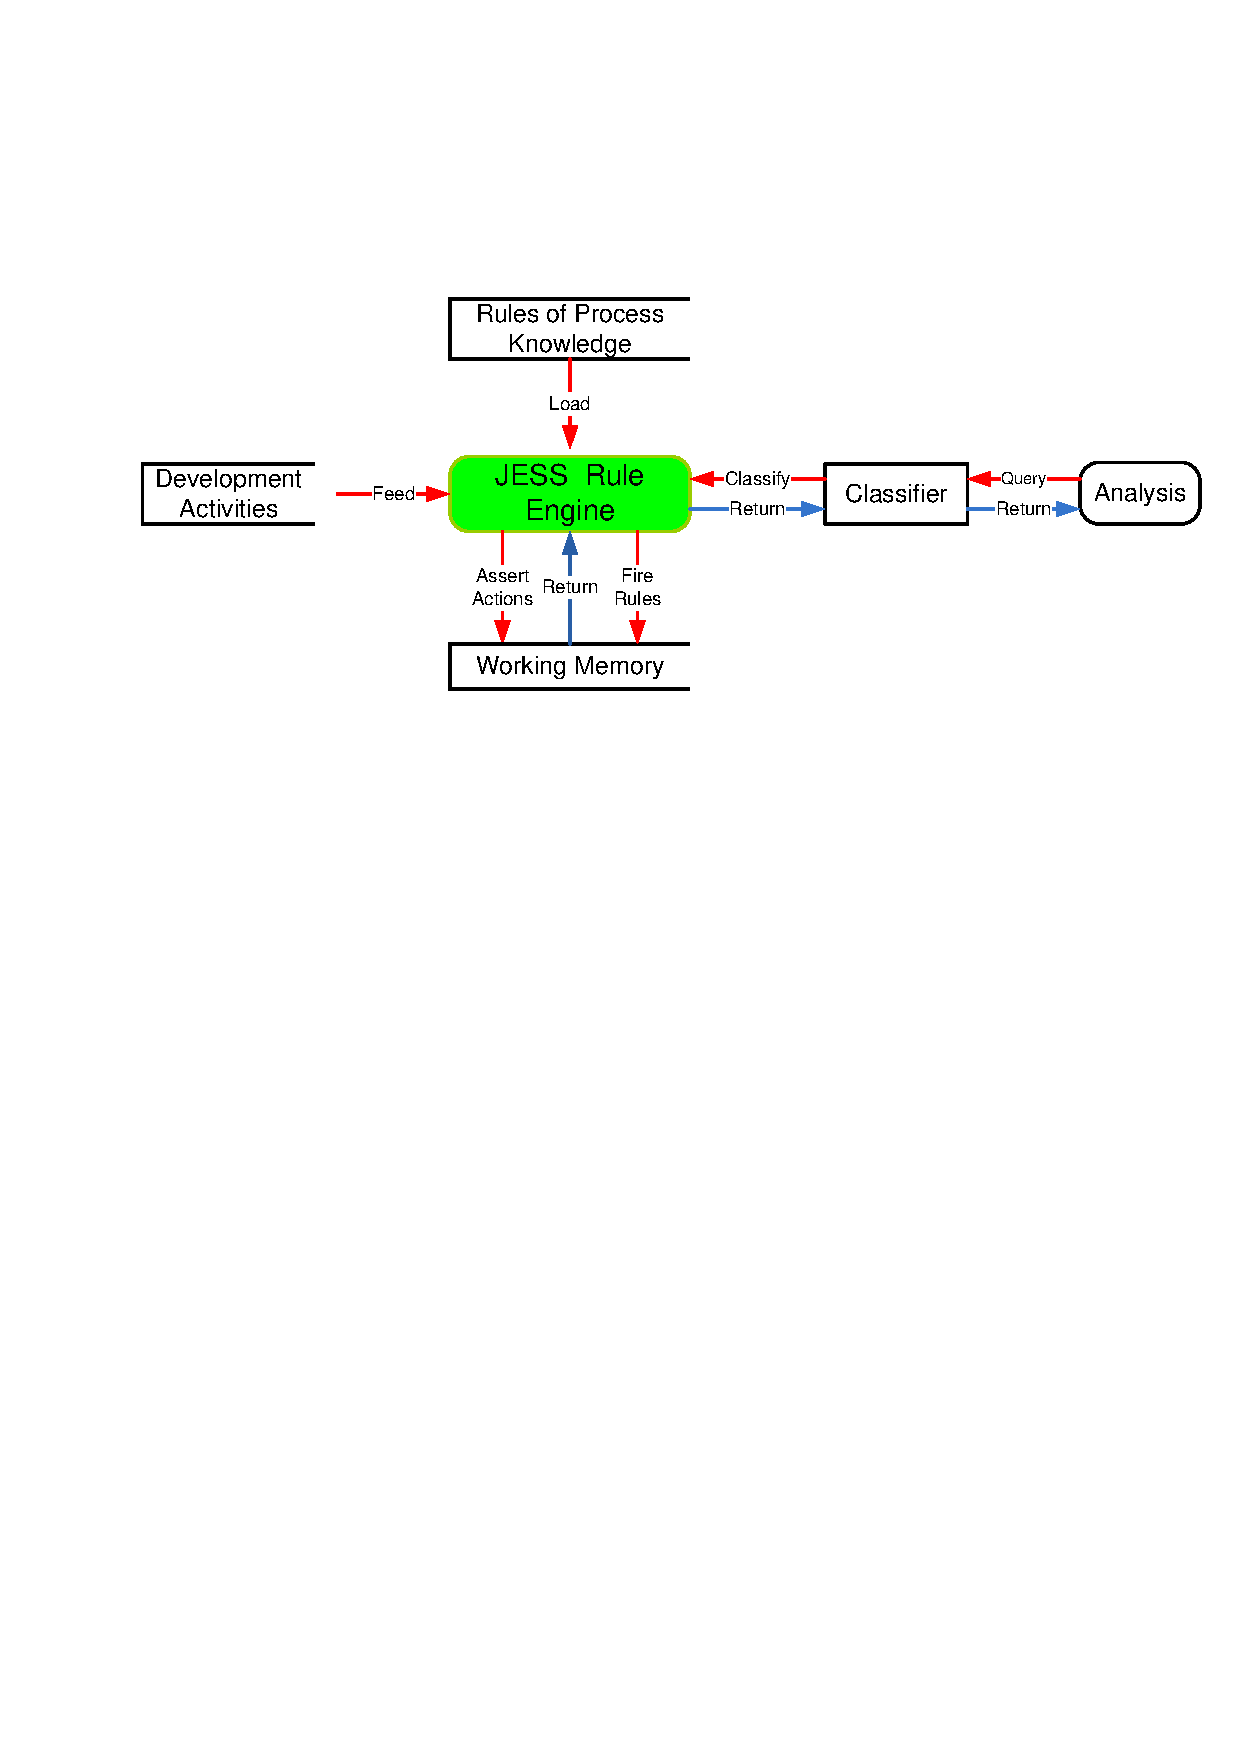
\includegraphics[width=1.0\textwidth]{figs/Visio-SDSA-BehaviorInference}
  \caption{Developer Behavior Inference}
  \label{fig:SDSA-Inference}
\end{figure}

The inference process is a mix of top-down and bottom-up 
methods. For the process of interest, developers can convert
the process knowledge into a set of rules, which are then fed 
into JESS's working memory. JESS can infer development behavior 
after all development actions in an episode are asserted in 
JESS as facts. Inferred results can be queried by applications 
via a classifier, the interface between JESS and SDSA.

\subsection{An Example}
\label{sec:SDSA-Example}
Now that we have shown how SDSA uses software process and 
product metrics for development behavior inference, I will 
use an example to demonstrate it. Figure \ref{fig:SDSA-Example} 
illustrates the usage of SDSA for inferring development behaviors. 
\begin{figure}[htbp]
  \centering
  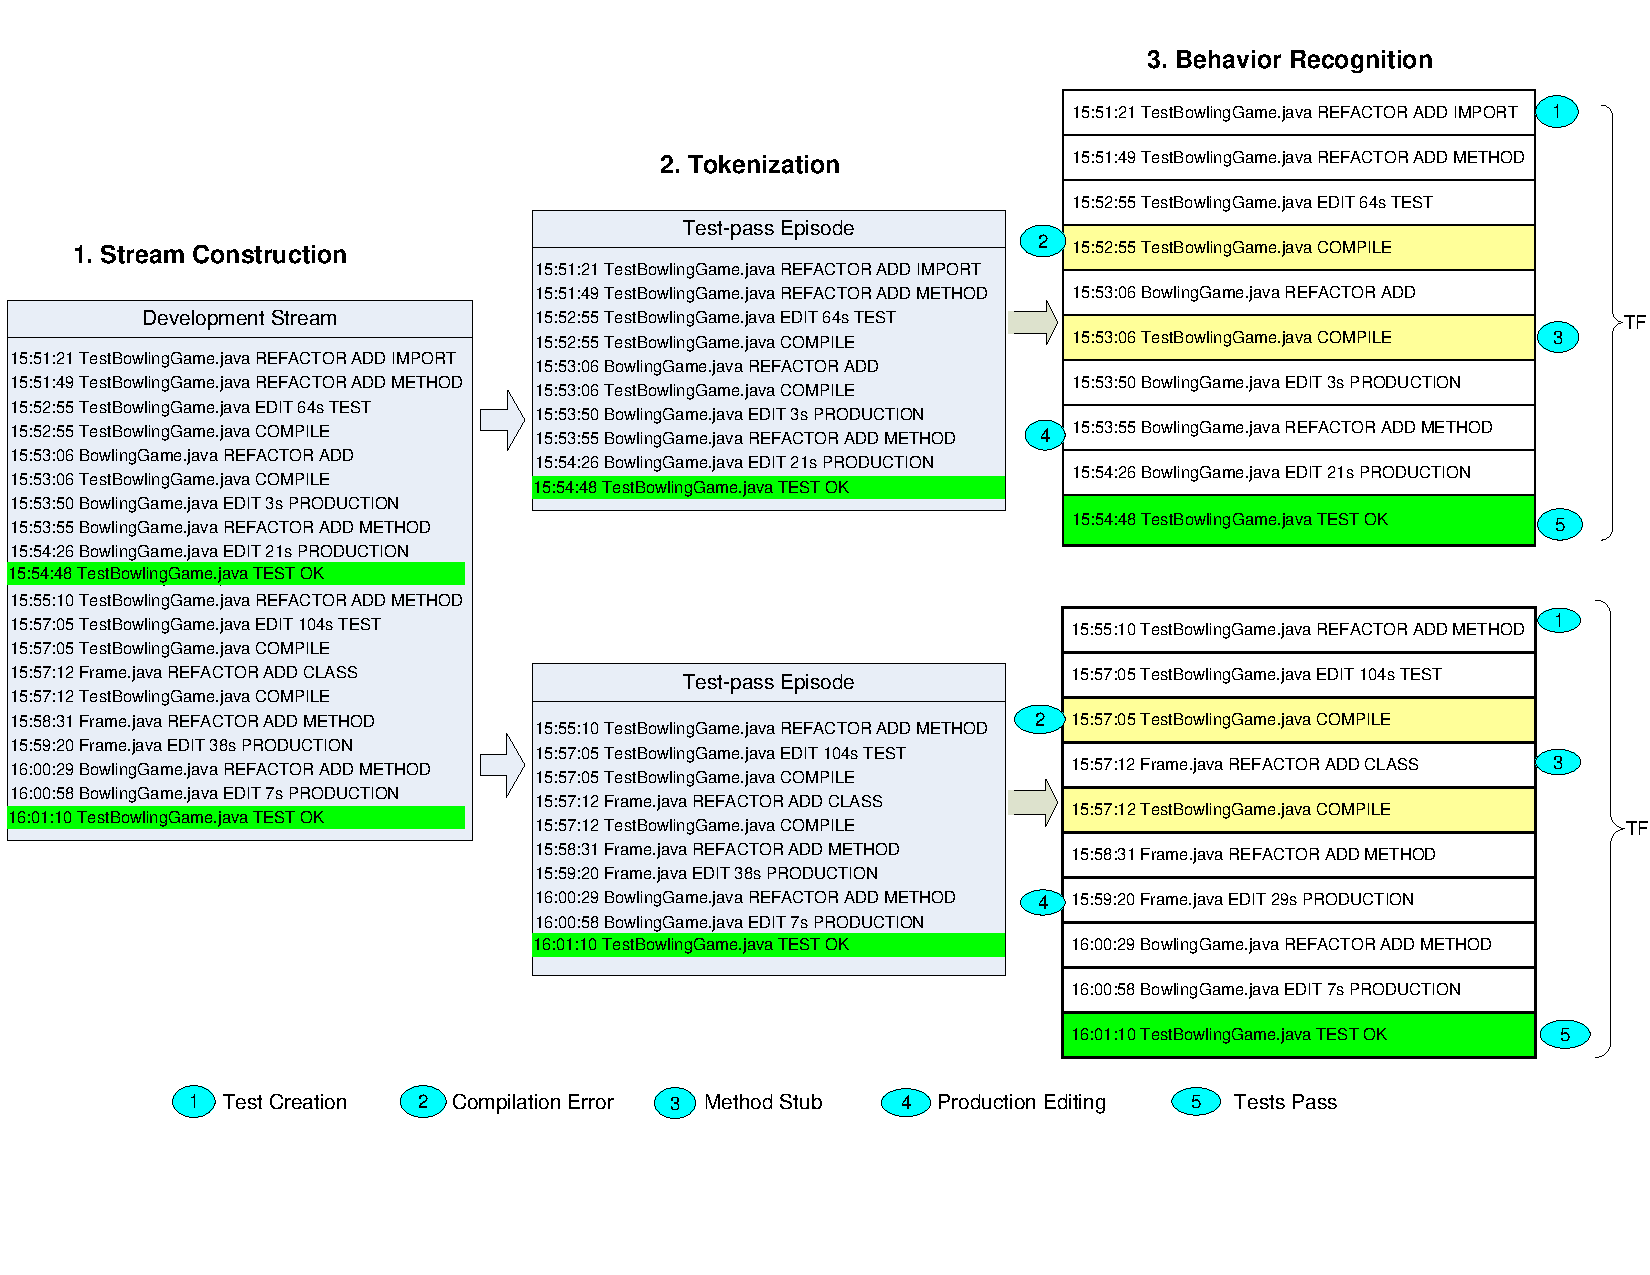
\includegraphics[width=1.0\textwidth]{figs/Visio-SDSA-Example}
  \caption{An SDSA Example}
  \label{fig:SDSA-Example}
\end{figure}
From 15:51:21 to 16:01:10, a developer implemented two user stories
of the bowling game in Test-Driven Development. We used Hackystat 
to instrument the development process and collected software process 
metrics including refactoring, editing, compilation and test 
invocations. Following the development stream construction method
described in Section \ref{sec:SDSA-Construction}, they were read 
and converted into development actions for construction of the
development stream. Part 1 of Figure \ref{fig:SDSA-Example} 
illustrates the internal structure of the development stream
that has 21 development actions. Among them, two are successful
test invocations that are painted in green background. Then, 
in part 2 of Figure \ref{fig:SDSA-Example}, SDSA's 
``Test Pass Tokenizer'' (See Section \ref{sec:SDSA-Partition}) 
was used to partition the development stream into two episodes. 
Further, development actions in the first episode were fed into
JESS to evaluate using an interface provided by SDSA. In part 3 
of Figure \ref{fig:SDSA-Example}, the inference rules detected 
a sequence of development activities that were in the order of 
(1) test creation, (2) compilation failures on test code, 
(3) method stub of production code, (4) production code editing, 
and (5) successful test invocation. Thus the development behavior 
in the first episode was recognized as ``TF'', a short name of 
Test-First. Similarly, the second episode was also recognized 
as ``TF'' by the inference rules.

%In this example, SDSA constructed a development stream on the 
%left-hand side, partitioned it into two episodes using the 
%``test pass'' tokenizer, and inferred that the development 
%behaviors in both episodes are a type of ``TF''. 

\section{Chapter Summary}
In this chapter, I first introduced Hackystat, a generic 
framework for software metrics collection and analyses, 
which makes it possible to design the SDSA framework for 
studying low-level software processes. SDSA has three 
sub-processes: (1) software development stream construction, 
(2) software development stream partition, and (3) 
development behavior inference. SDSA is configurable 
and extensible. I concluded this chapter with an example 
in Section \ref{sec:SDSA-Example} using a portion of a 
development stream developed in TDD. 